\section{Оборудование}
Для измерения концентрации используются датчики теплопроводности. При этом используется, что
теплопроводность $\kappa$ смеси зависит от ее состава:
\[\Delta \kappa\approx C\Delta n\]

Сами датчики теплопроводности устроены следующим образом. Тонкая
платиновая проволочка, протянутая вдоль оси стеклянного цилиндра,
нагревается током. Внутренняя полость датчика сообщается с объёмом
камеры через отверстия, размеры которых таковы, что скорость диффузии
из объёма сосуда в полость датчика значительно больше скорости диффузии
из одного объёма в другой. Таким образом, состав газа в датчике практически
совпадает с составом газа в объёме. Тепло от проволочки к стенке
цилиндра передаётся главным образом за счёт теплопроводности газа, находящегося
внутри цилиндра. При заданной мощности нагревания приращение температуры
проволочки и, следовательно, приращение её сопротивления пропорциональны
теплопроводности газа.

Для измерения сопротивлений используется мостовая схема, позволяющая
определять разность показаний датчиков с высокой точностью.
Мост балансируется при заполнении сосудов (и датчиков) одной и той же
смесью. При заполнении сосудов смесями различного состава возникает
<<разбаланc>> моста.
\[U\varpropto \Delta\kappa \varpropto \Delta n\]
\[U=U_0\exp\left(-\frac{t}{\tau}\right)\]

Измеряя $U(t)$, можно получить $\tau$, а из него~--- коэффициент диффузии.

\begin{figure}[ht!]
    \centering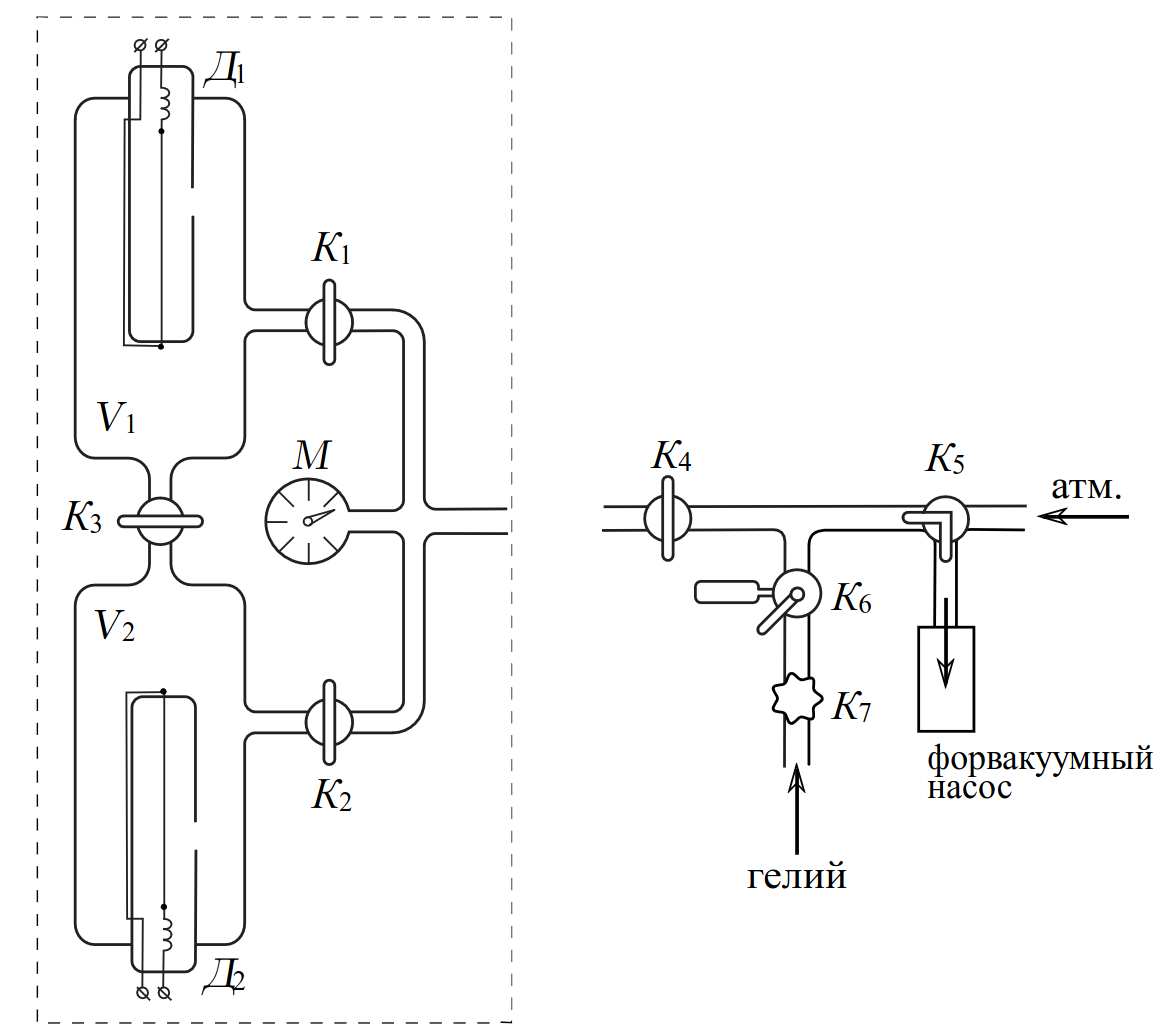
\includegraphics[width=0.8\linewidth]{img/eq1.png}
\end{figure}

Схема установки приведена на рисунке. Для откачки используется форвакуумный насос.

Измерительная часть состоит из сосудов $V_2$ и $V_1$, для их накачки служат краны
К1 и К2. Кран К3 открывается для начала диффузии. Для накачки гелия используются
краны К6 и К7.

Датчики теплопроводности Д1 и Д2 расположены в сосудах и включены в мостовую схему.
\begin{figure}[ht!]
    \centering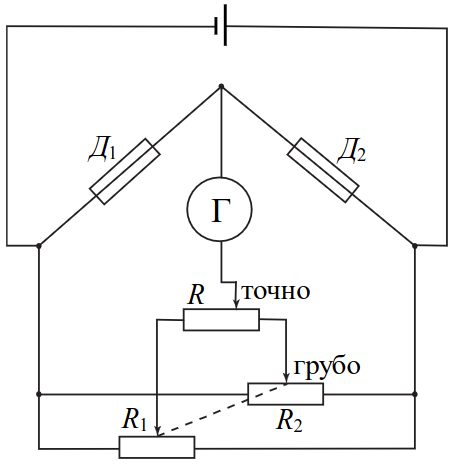
\includegraphics[width=0.4\linewidth]{img/eq2.png}
\end{figure}

В одну из диагоналей
моста включён высокочувствительный
вольтметр (гальванометр) Г, к другой подключается источник небольшого постоянного
напряжения. Сопротивления проволок датчиков составляют одно из плеч моста. Второе
плечо составляют переменные сопротивления
$R_1$, $R_2$ и $R$, служащие для установки показаний вольтметра Г на нуль
(балансировка моста). Сопротивления $R_1$ и $R_2$ спарены (их подвижные контакты находятся
на общей оси) и изменяются одновременно при повороте ручки грубой
регулировки. Точная балансировка выполняется потенциометром $R$. Балансировку
необходимо проводить перед каждым экспериментом заново: при
этом установка заполняется чистым газом (воздухом без гелия) при давлении, близком
<<рабочему>> (при котором затем будут проводится измерения).
